% #############################################################################
% This is Chapter 3
% !TEX root = ../main.tex
% #############################################################################
% Change the Name of the Chapter i the following line
\fancychapter{This is the Third Chapter}
\cleardoublepage
% The following line allows to ref this chapter
\label{chap:architecture}

Donec gravida posuere arcu. Nulla facilisi. Phasellus imperdiet. Vestibulum at metus. Integer euismod. Nullam placerat rhoncus sapien. Ut euismod. Praesent libero. Morbi pellentesque libero sit amet ante. Maecenas tellus. Maecenas erat. Pellentesque habitant morbi tristique senectus et netus et malesuada fames ac turpis egestas.
% #############################################################################
\section{Architecture Design Requirements} 
\textcolor{violet}{Example of a Flowchart for a system, in \Cref{fig:flowchart}, created with \url{https://www.draw.io} and then exported as ``PDF'' crop format (a true vector image that can be scaled to no end, with no pixels or distortion).}

\begin{figure}[h]
\centering
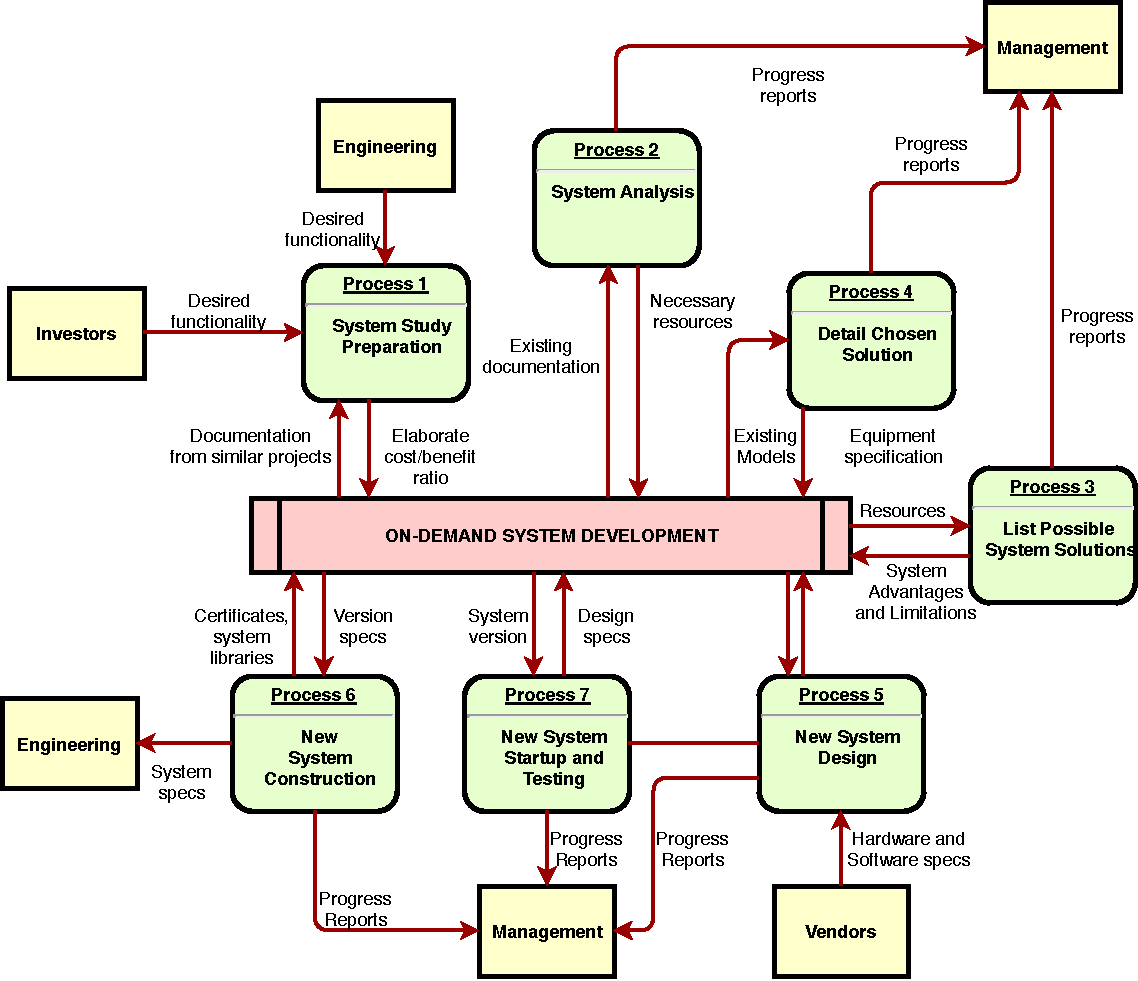
\includegraphics[width=1.0\textwidth]{./Images/Flowchart_from_draw-io.pdf}
\caption{System Processes}
\label{fig:flowchart}
\end{figure}

Quisque facilisis erat a dui. Nam malesuada ornare dolor. Cras gravida, diam sit amet rhoncus ornare, erat elit consectetuer erat, id egestas pede nibh eget odio. Proin tincidunt, velit vel porta elementum, magna diam molestie sapien, non aliquet massa pede eu diam. Aliquam iaculis. Fusce et ipsum et nulla tristique facilisis. Donec eget sem sit amet ligula viverra gravida. Etiam vehicula urna vel turpis. 

\textcolor{violet}{And here another diagram of a network (\Cref{fig:network}) created with \url{https://www.draw.io} and then exported as ``PDF'' crop format.}

\begin{figure}[h]
\centering
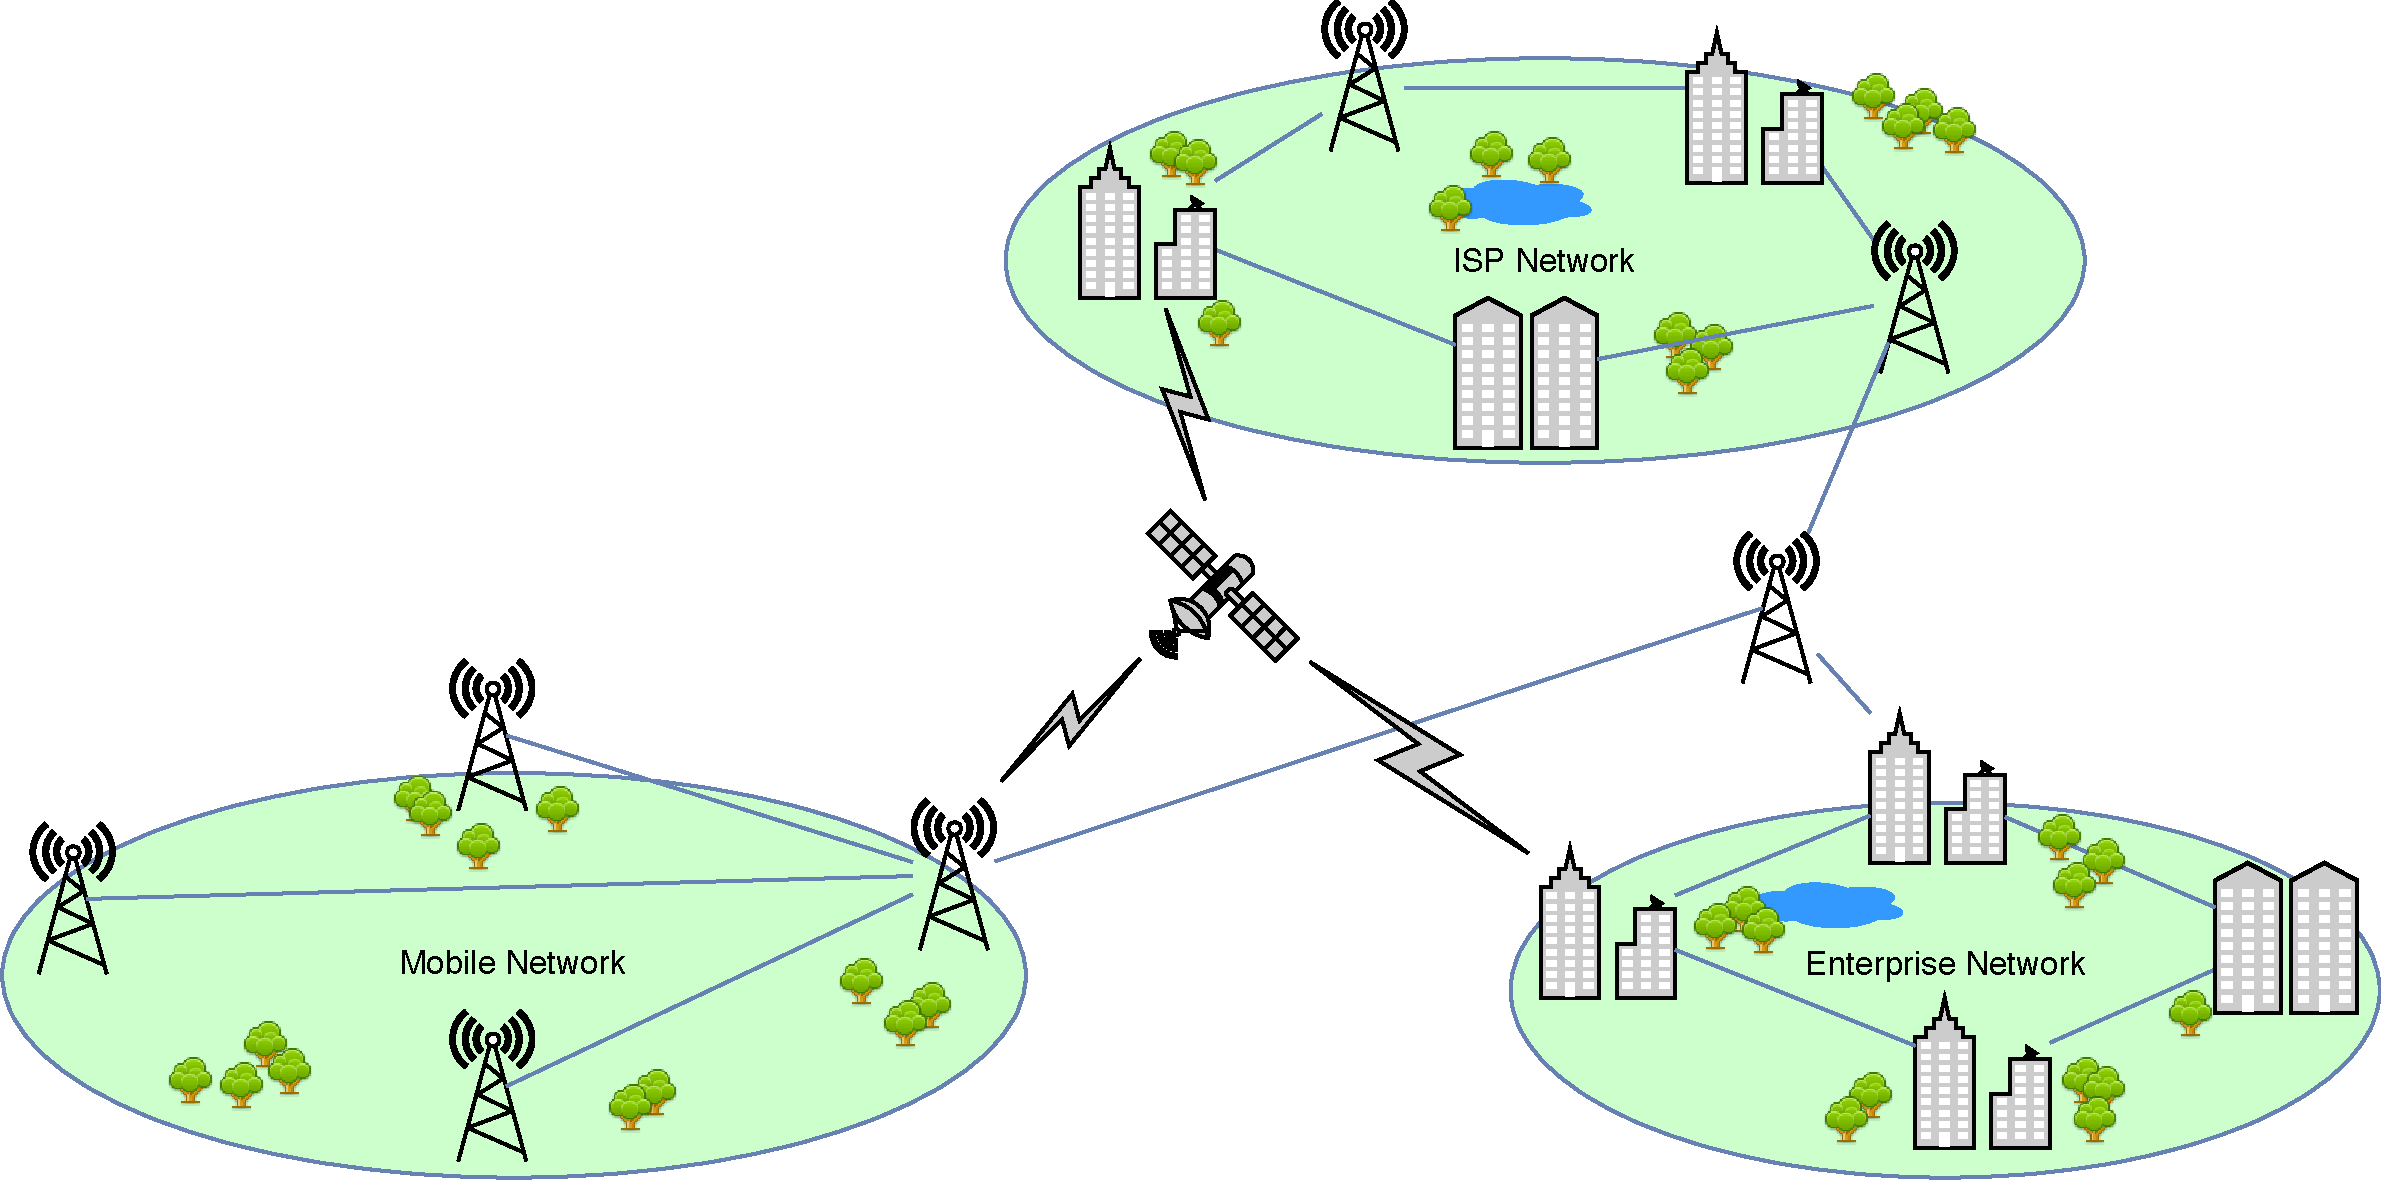
\includegraphics[width=1.0\textwidth]{./Images/Network_from_draw-io.pdf}
\caption{Network Diagram}
\label{fig:network}
\end{figure}

Suspendisse sagittis ante a urna. Morbi a est quis orci consequat rutrum. Nullam egestas feugiat felis. Integer adipiscing semper ligula. Nunc molestie, nisl sit amet cursus convallis, sapien lectus pretium metus, vitae pretium enim wisi id lectus. Donec vestibulum. Etiam vel nibh. Nulla facilisi. Mauris pharetra. Donec augue. Fusce ultrices, neque id dignissim ultrices, tellus mauris dictum elit, vel lacinia enim metus eu nunc:

\begin{description}
	\item[\textbf{Web-streaming:}]
	The client application should support streaming media using \ac{HTTP} protocols.
	\item[\textbf{Multi-source streaming:}]
	The client application should support multi-source streaming media, i.e., ``simultaneous'' streaming of media content components from a network, supported\slash complemented by \ac{CDN}\slash \ac{CC} services. 
	\item[\textbf{Support content Metadata Description:}]
	The client application should support content metadata description in a format similar or compliant with MPEG \ac{DASH} \cite{ISO/IEC:2012fk}. 
	\item[\textbf{Scalable and Adaptive Media Contents:}]
	The system should support on-demand streaming of scalable and adaptive contents based on \ac{SVC}.
	\item[\textbf{Heterogenous End-User Devices:}]
	The client application should be compatible with current and future generations of end-user devices form factors, irrespective of their performance, screen size and resolution.
	\item[\textbf{Access Network independency:}] 
	The solution should provide the expected service over different types of access networks supported by the end-user devices, such as Wireless \acp{LAN} (IEEE 802.11) or cellular data networks such as \ac{GPRS}, \ac{UMTS}, \ac{LTE}, etc.
\end{description}

Cras gravida, diam sit amet rhoncus ornare, erat elit consectetuer erat, id egestas pede nibh eget odio. Proin tincidunt, velit vel porta elementum, magna diam molestie sapien, non aliquet massa pede eu diam. Aliquam iaculis. Fusce et ipsum et nulla tristique facilisis.
% #############################################################################
\section{Architecture Design Requirements}
Ut nulla. Vivamus bibendum, nulla ut congue fringilla, lorem ipsum ultricies risus, ut rutrum velit tortor vel purus. In hac habitasse platea dictumst. Duis fermentum, metus sed congue gravida, arcu dui ornare urna, ut imperdiet enim odio dignissim ipsum. Nulla facilisi. Cras magna ante, bibendum sit amet, porta vitae, laoreet ut, justo. Nam tortor sapien, pulvinar nec, malesuada in, ultrices in, tortor. Cras ultricies placerat eros. Quisque odio eros, feugiat non, iaculis nec, lobortis sed, arcu. Pellentesque sit amet sem et purus pretium consectetuer \Cref{mpd}\todo[color=cyan!40, author=RC, fancyline]{A listing for XML code, with syntax highlighting}{}.

\begin{minipage}[c]{0.95\textwidth}
\begin{center}
\begin{spacing}{0.5}
\begin{lstlisting}[frame=lines,style=XML,caption={Example of a MPD file.},label=mpd]
<?xml version="1.0" encoding="UTF-8"?>
<StreamInfo version="2.0">
    <Clip duration="PT01M0.00S">
        <BaseURL>videos/</BaseURL>
        <Description>svc_1</Description>
        <Representation mimeType="video/SVC" codecs="svc" frameRate="30.00" bandwidth="401.90"
            width="176" height="144" id="L0">
            <BaseURL>svc_1/</BaseURL>
            <SegmentInfo from="0" to="11" duration="PT5.00S">
                <BaseURL>svc_1-L0-</BaseURL>
            </SegmentInfo>
        </Representation>
        <Representation mimeType="video/SVC" codecs="svc" frameRate="30.00" bandwidth="1322.60"
            width="352" height="288" id="L1">
            <BaseURL>svc_1/</BaseURL>
            <SegmentInfo from="0" to="11" duration="PT5.00S">
                <BaseURL>svc_1-L1-</BaseURL>
            </SegmentInfo>
        </Representation>
    </Clip>
</StreamInfo>
\end{lstlisting}
\end{spacing}
\end{center}
\end{minipage}

Nam malesuada ornare dolor. Cras gravida, diam sit amet rhoncus ornare, erat elit consectetuer erat, id egestas pede nibh eget odio. Proin tincidunt, velit vel porta elementum, magna diam molestie sapien, non aliquet massa pede eu diam.